\documentclass[]{article}
\usepackage[left=1in,top=1in,right=1in,bottom=1in]{geometry}


%%%% more monte %%%%
% thispagestyle{empty}
% https://stackoverflow.com/questions/2166557/how-to-hide-the-page-number-in-latex-on-first-page-of-a-chapter
\usepackage{color}
% \usepackage[table]{xcolor} % are they using color?

% \definecolor{WSU.crimson}{HTML}{981e32}
% \definecolor{WSU.gray}{HTML}{5e6a71}

% \definecolor{shadecolor}{RGB}{248,248,248}
\definecolor{WSU.crimson}{RGB}{152,30,50} % use http://colors.mshaffer.com to convert from 981e32
\definecolor{WSU.gray}{RGB}{94,106,113}

%%%%%%%%%%%%%%%%%%%%%%%%%%%%

\newcommand*{\authorfont}{\fontfamily{phv}\selectfont}
\usepackage{lmodern}


  \usepackage[T1]{fontenc}
  \usepackage[utf8]{inputenc}




\usepackage{abstract}
\renewcommand{\abstractname}{}    % clear the title
\renewcommand{\absnamepos}{empty} % originally center

\renewenvironment{abstract}
 {{%
    \setlength{\leftmargin}{0mm}
    \setlength{\rightmargin}{\leftmargin}%
  }%
  \relax}
 {\endlist}

\makeatletter
\def\@maketitle{%
  \pagestyle{empty}
  \newpage
%  \null
%  \vskip 2em%
%  \begin{center}%
  \let \footnote \thanks
    {\fontsize{18}{20}\selectfont\raggedright  \setlength{\parindent}{0pt} \@title \par}%
}
%\fi
\makeatother






\usepackage{color}
\usepackage{fancyvrb}
\newcommand{\VerbBar}{|}
\newcommand{\VERB}{\Verb[commandchars=\\\{\}]}
\DefineVerbatimEnvironment{Highlighting}{Verbatim}{commandchars=\\\{\}}
% Add ',fontsize=\small' for more characters per line
\usepackage{framed}
\definecolor{shadecolor}{RGB}{248,248,248}
\newenvironment{Shaded}{\begin{snugshade}}{\end{snugshade}}
\newcommand{\AlertTok}[1]{\textcolor[rgb]{0.94,0.16,0.16}{#1}}
\newcommand{\AnnotationTok}[1]{\textcolor[rgb]{0.56,0.35,0.01}{\textbf{\textit{#1}}}}
\newcommand{\AttributeTok}[1]{\textcolor[rgb]{0.77,0.63,0.00}{#1}}
\newcommand{\BaseNTok}[1]{\textcolor[rgb]{0.00,0.00,0.81}{#1}}
\newcommand{\BuiltInTok}[1]{#1}
\newcommand{\CharTok}[1]{\textcolor[rgb]{0.31,0.60,0.02}{#1}}
\newcommand{\CommentTok}[1]{\textcolor[rgb]{0.56,0.35,0.01}{\textit{#1}}}
\newcommand{\CommentVarTok}[1]{\textcolor[rgb]{0.56,0.35,0.01}{\textbf{\textit{#1}}}}
\newcommand{\ConstantTok}[1]{\textcolor[rgb]{0.00,0.00,0.00}{#1}}
\newcommand{\ControlFlowTok}[1]{\textcolor[rgb]{0.13,0.29,0.53}{\textbf{#1}}}
\newcommand{\DataTypeTok}[1]{\textcolor[rgb]{0.13,0.29,0.53}{#1}}
\newcommand{\DecValTok}[1]{\textcolor[rgb]{0.00,0.00,0.81}{#1}}
\newcommand{\DocumentationTok}[1]{\textcolor[rgb]{0.56,0.35,0.01}{\textbf{\textit{#1}}}}
\newcommand{\ErrorTok}[1]{\textcolor[rgb]{0.64,0.00,0.00}{\textbf{#1}}}
\newcommand{\ExtensionTok}[1]{#1}
\newcommand{\FloatTok}[1]{\textcolor[rgb]{0.00,0.00,0.81}{#1}}
\newcommand{\FunctionTok}[1]{\textcolor[rgb]{0.00,0.00,0.00}{#1}}
\newcommand{\ImportTok}[1]{#1}
\newcommand{\InformationTok}[1]{\textcolor[rgb]{0.56,0.35,0.01}{\textbf{\textit{#1}}}}
\newcommand{\KeywordTok}[1]{\textcolor[rgb]{0.13,0.29,0.53}{\textbf{#1}}}
\newcommand{\NormalTok}[1]{#1}
\newcommand{\OperatorTok}[1]{\textcolor[rgb]{0.81,0.36,0.00}{\textbf{#1}}}
\newcommand{\OtherTok}[1]{\textcolor[rgb]{0.56,0.35,0.01}{#1}}
\newcommand{\PreprocessorTok}[1]{\textcolor[rgb]{0.56,0.35,0.01}{\textit{#1}}}
\newcommand{\RegionMarkerTok}[1]{#1}
\newcommand{\SpecialCharTok}[1]{\textcolor[rgb]{0.00,0.00,0.00}{#1}}
\newcommand{\SpecialStringTok}[1]{\textcolor[rgb]{0.31,0.60,0.02}{#1}}
\newcommand{\StringTok}[1]{\textcolor[rgb]{0.31,0.60,0.02}{#1}}
\newcommand{\VariableTok}[1]{\textcolor[rgb]{0.00,0.00,0.00}{#1}}
\newcommand{\VerbatimStringTok}[1]{\textcolor[rgb]{0.31,0.60,0.02}{#1}}
\newcommand{\WarningTok}[1]{\textcolor[rgb]{0.56,0.35,0.01}{\textbf{\textit{#1}}}}



\title{\textbf{\textcolor{WSU.crimson}{A boring (academic) title or a clever title?}} \newline \textbf{\textcolor{WSU.gray}{A secondary title}}  }

%  

% \author{ \Large true \hfill \normalsize \emph{} }
\author{\Large Connor StarrHurst\vspace{0.05in} \newline\normalsize\emph{Washington State University}  }


\date{November 10, 2020}
\setcounter{secnumdepth}{3}

\usepackage{titlesec}
% See the link above: KOMA classes are not compatible with titlesec any more. Sorry.
% https://github.com/jbezos/titlesec/issues/11
\titleformat*{\section}{\bfseries}
\titleformat*{\subsection}{\bfseries\itshape}
\titleformat*{\subsubsection}{\itshape}
\titleformat*{\paragraph}{\itshape}
\titleformat*{\subparagraph}{\itshape}

% https://code.usgs.gov/usgs/norock/irvine_k/ip-092225/


%\titleformat*{\section}{\normalsize\bfseries}
%\titleformat*{\subsection}{\normalsize\itshape}
%\titleformat*{\subsubsection}{\normalsize\itshape}
%\titleformat*{\paragraph}{\normalsize\itshape}
%\titleformat*{\subparagraph}{\normalsize\itshape}

% https://tex.stackexchange.com/questions/233866/one-column-multicol-environment#233904
\usepackage{environ}
\NewEnviron{auxmulticols}[1]{%
  \ifnum#1<2\relax% Fewer than 2 columns
    %\vspace{-\baselineskip}% Possible vertical correction
    \BODY
  \else% More than 1 column
    \begin{multicols}{#1}
      \BODY
    \end{multicols}%
  \fi
}





\usepackage{natbib}
\setcitestyle{aysep={}} %% no year, comma just year
% \usepackage[numbers]{natbib}
\bibliographystyle{./../biblio/ormsv080.bst}



\usepackage[strings]{underscore} % protect underscores in most circumstances




\newtheorem{hypothesis}{Hypothesis}
\usepackage{setspace}


%%%%%%%%%%%%%%%%%%%%%%%%%%%%%%%%%%%%%%%%%%%%%%%%%%%%%
%%% MONTE ADDS %%%

\usepackage{fancyhdr} % fancy header 
\usepackage{lastpage} % last page 

\usepackage{multicol}


\usepackage{etoolbox}
\AtBeginEnvironment{quote}{\singlespacing\small}
% https://tex.stackexchange.com/questions/325695/how-to-style-blockquote


\usepackage{soul}			%% allows strike-through
\usepackage{url}			%% fixes underscores in urls
\usepackage{csquotes}		%% allows \textquote in references
\usepackage{rotating}		%% allows table and box rotation
\usepackage{caption}		%% customize caption information
\usepackage{booktabs}		%% enhance table/tabular environment
\usepackage{tabularx}		%% width attributes updates tabular
\usepackage{enumerate}		%% special item environment
\usepackage{enumitem}		%% special item environment

\usepackage{lineno}		%% allows linenumbers for editing using \linenumbers
\usepackage{hanging}


\usepackage{mathtools}  	%% also loads amsmath
\usepackage{bm}		%% bold-math
\usepackage{scalerel}	%% scale one element (make one beta bigger font)

\newcommand{\gFrac}[2]{ \genfrac{}{}{0pt}{1}{{#1}}{#2} }

\newcommand{\betaSH}[3]{  \gFrac{\text{\tiny #1}}{{\text{\tiny #2}}}\hat{\beta}_{\text{#3}}   }
\newcommand{\betaSB}[3]{              ^{\text{#1}} _{\text{#2}} \bm{\beta} _{\text{#3}}                   }  %% bold
\newcommand{\bigEQ}{  \scaleobj{1.5}{{\ }= } }
\newcommand{\bigP}[1]{  \scaleobj{1.5}{#1 } }





\usepackage{endnotes}  % he already does this ...
\renewcommand{\enotesize}{\normalsize}
% https://tex.stackexchange.com/questions/99984/endnotes-do-not-be-superscript-and-add-a-space
\renewcommand\makeenmark{\textsuperscript{[\theenmark]}} % in brackets %
% https://tex.stackexchange.com/questions/31574/how-to-control-the-indent-in-endnotes
\patchcmd{\enoteformat}{1.8em}{0pt}{}{}

\patchcmd{\theendnotes}
  {\makeatletter}
  {\makeatletter\renewcommand\makeenmark{\textbf{[\theenmark]} }}
  {}{}



% https://tex.stackexchange.com/questions/141906/configuring-footnote-position-and-spacing

\addtolength{\footnotesep}{5mm} % change to 1mm

\renewcommand{\thefootnote}{\textbf{\arabic{footnote}}}
\let\footnote=\endnote
%\renewcommand*{\theendnote}{\alph{endnote}}
%\renewcommand{\theendnote}{\textbf{\arabic{endnote}}}


\renewcommand*{\notesname}{ENDNOTES}

\makeatletter
\def\enoteheading{\section*{\notesname
  \@mkboth{\MakeUppercase{\notesname}}{\MakeUppercase{\notesname}}}%
  \mbox{}\par\vskip-2.3\baselineskip\noindent\rule{.5\textwidth}{0.4pt}\par\vskip\baselineskip}
\makeatother


\renewcommand*{\contentsname}{TABLE OF CONTENTS}

\renewcommand*{\refname}{REFERENCES}


%\usepackage{subfigure}
\usepackage{subcaption}

\captionsetup{labelfont=bf}  % Make Table / Figure bold

%%% you could add elements here ... monte says .... %%%
%\usepackage{mypackageForCapitalH}


%%%%%%%%%%%%%%%%%%%%%%%%%%%%%%%%%%%%%%%%%%%%%%%%%%%%%

% set default figure placement to htbp
\makeatletter
\def\fps@figure{htbp}
\makeatother


% move the hyperref stuff down here, after header-includes, to allow for - \usepackage{hyperref}

\makeatletter
\@ifpackageloaded{hyperref}{}{%
\ifxetex
  \PassOptionsToPackage{hyphens}{url}\usepackage[setpagesize=false, % page size defined by xetex
              unicode=false, % unicode breaks when used with xetex
              xetex]{hyperref}
\else
  \PassOptionsToPackage{hyphens}{url}\usepackage[draft,unicode=true]{hyperref}
\fi
}

\@ifpackageloaded{color}{
    \PassOptionsToPackage{usenames,dvipsnames}{color}
}{%
    \usepackage[usenames,dvipsnames]{color}
}
\makeatother
\hypersetup{breaklinks=true,
            bookmarks=true,
            pdfauthor={Connor StarrHurst (Washington State University)},
             pdfkeywords = {multiple comparisons to control; multivariate chi-square distribution;
nonlinear growth curves; Richard's curve; simulated critical points},  
            pdftitle={A boring (academic) title or a clever title?: A secondary title},
            colorlinks=true,
            citecolor=blue,
            urlcolor=blue,
            linkcolor=magenta,
            pdfborder={0 0 0}}
\urlstyle{same}  % don't use monospace font for urls

% Add an option for endnotes. -----

%
% add tightlist ----------
\providecommand{\tightlist}{%
\setlength{\itemsep}{0pt}\setlength{\parskip}{0pt}}

% add some other packages ----------

% \usepackage{multicol}
% This should regulate where figures float
% See: https://tex.stackexchange.com/questions/2275/keeping-tables-figures-close-to-where-they-are-mentioned
\usepackage[section]{placeins}



\pagestyle{fancy}   
\lhead{\textcolor{WSU.crimson}{\textbf{ A boring (academic) title or a clever title? }}}
\chead{}
\rhead{\textcolor{WSU.gray}{\textbf{  Page\ \thepage\ of\ \protect\pageref{LastPage} }}}
\lfoot{}
\cfoot{}
\rfoot{}


\begin{document}
	
% \pagenumbering{arabic}% resets `page` counter to 1 
%
% \maketitle

{% \usefont{T1}{pnc}{m}{n}
\setlength{\parindent}{0pt}
\thispagestyle{plain}
{\fontsize{18}{20}\selectfont\raggedright 
\maketitle  % title \par  

}

{
   \vskip 13.5pt\relax \normalsize\fontsize{11}{12} 
   
\textbf{\authorfont Connor StarrHurst} \hskip 15pt \emph{\small Washington State University}   

}

}








\begin{abstract}

    \hbox{\vrule height .2pt width 39.14pc}

    \vskip 8.5pt % \small 

\noindent In this article we compare the \emph{empirical characteristic function}
\citep{Tukey:1977, Becker:1988} to a
\emph{moment-generating-functional form} to compute the proportion of
hypotheses \(m\) that are rejected under the null hypothesis.
\vspace{0.25in}

\noindent Here is a second paragraph of the abstract (if necessary), and
with the pipe notation it doesn't break. Notice it still needs to be
indented. \vspace{0.25in}

\noindent Generally, we write this abstract last. Often it is called the
executive summary. It should succinctly summarize the entire document.
You can include references such as this one to the Appendices section
\ref{sec:appendix} if necessary.


\vskip 8.5pt \noindent \textbf{\underline{Keywords}:} multiple comparisons to control; multivariate chi-square distribution;
nonlinear growth curves; Richard's curve; simulated critical points \par

    




    
    \hbox{\vrule height .2pt width 39.14pc}
    \vskip 5pt 
    \hfill \textbf{\textcolor{WSU.gray}{ November 10, 2020 } }
    \vskip 5pt 
    
\end{abstract}


\vskip -8.5pt



 % removetitleabstract

\noindent  

\section{Introduction}
\label{sec:intro}

Write something here.

{[}ONE GRAPHIC{]}

{[}TWO GRAPHICS AS ONE{]}

Write something here.

\section{Research Question:  What is my primary question}
\label{sec:rq}

\subsection{What is my secondary question}
\label{sec:rq2}

\subsection{What is my other secondary question}
\label{sec:rq3}

\section{Data Description}
\label{sec:data}

Very brief introduction to the data, how it was collected, and so on.
Remember that everything is covered (who, what, when, where, why, how,
so what, and so on). Reference the section in the Appendix with greater
detail about the data provenance. This section should be about two
paragraphs, and the Appendix should have more information.

\subsection{Summary of Sample}
\label{sec:data-sample}

\subsection{Summary Statistics of Data}
\label{sec:data-summary}

\section{Key Findings}
\label{sec:findings}

\section{Conclusion}
\label{sec:conclusion}

\newpage

This was a new page

This is a newline. \newline  Here is some more text.

Below are some example code that may benefit you in preparing your
document. \newline

\vspace{0.25in}

\noindent Please state your name: \hrulefill \newline I was born on
\hrulefill in \hrulefill \vspace{0.25in}

\begin{equation}
\label{eq:my-model}
    Y_{jt} = \alpha + \bm{\beta}X_{jt} + \upsilon_{j}  + \varepsilon_{jt} ,
\end{equation}

\noindent where \(\alpha\) is the grand mean, \(\upsilon_{j}\) is the
fixed-time country mean, \(X_{jt}\) (country \(j\) at time \(t\)) is the
matrix of country-level observations for the vector of aforementioned
parameters \(\bm{\beta}\), and \(\varepsilon_{jt}\) represents the
residual idiosyncratic disturbance. Our panel data set consists of
repeated observations of countries over time. Therefore, we employ
cross-section time-series models. This approach redefines
Equation\textasciitilde{}\ref{eq:my-model} by subtracting time-demeaned
values. This \emph{within} transformation subtracts constant country
effects for the dependent variable \(\bar{Y_{j}}\), the predictor
variables \(\bar{X_{j}}\), and the intercept \(\bar{\upsilon_{j}}\):

\begin{equation}
\label{eq:my-random}
    (Y_{jt} - \theta \bar{Y_{j}}) = (1-\theta)\alpha + \bm{\beta}(X_{jt} - \bar{X_{j}}) +  (\upsilon_{jt} - \theta \bar{\upsilon_{j}})  ,
\end{equation}

\noindent If \(\theta = 0\), the model reduces to a basic pooled
ordinary-least-squares (OLS) model; if \(\theta = 1\), the model reduces
to a fixed-effects model; otherwise the model represents a
random-effects model. The pooled OLS estimation is biased if country
effects exist \citep{Hsiao:2003}. The random-effects model may be
susceptible to omitted-variable bias \citep{Wooldridge:2006}: bias
because a predictor was excluded from the model specification.
Conversely, the fixed-effects model is not susceptible to this bias as
it captures unobserved intracountry variation around its average
country-level ``fixed effect." Panel-data analysis commonly has issues
with heteroskedasticity, serial autocorrelation, and cross-sectional
autocorrelation.

\vspace{0.5in}

\(i=1\) and \[i = 1\]

\vspace{0.5in}

\begin{tabular}{ c c c c c}
  1 & 2 & 3 & 4 & 5 \\
  \hline
  6 & 7 & 8 & 9 & 10
\end{tabular}

\vspace{0.5in}

\begin{figure}[!ht]
%% figures have hrule, tables have hline
    \hrule
    \caption{ \textbf{Conceptual Model} }
    \begin{center}
        \scalebox{1.00}{    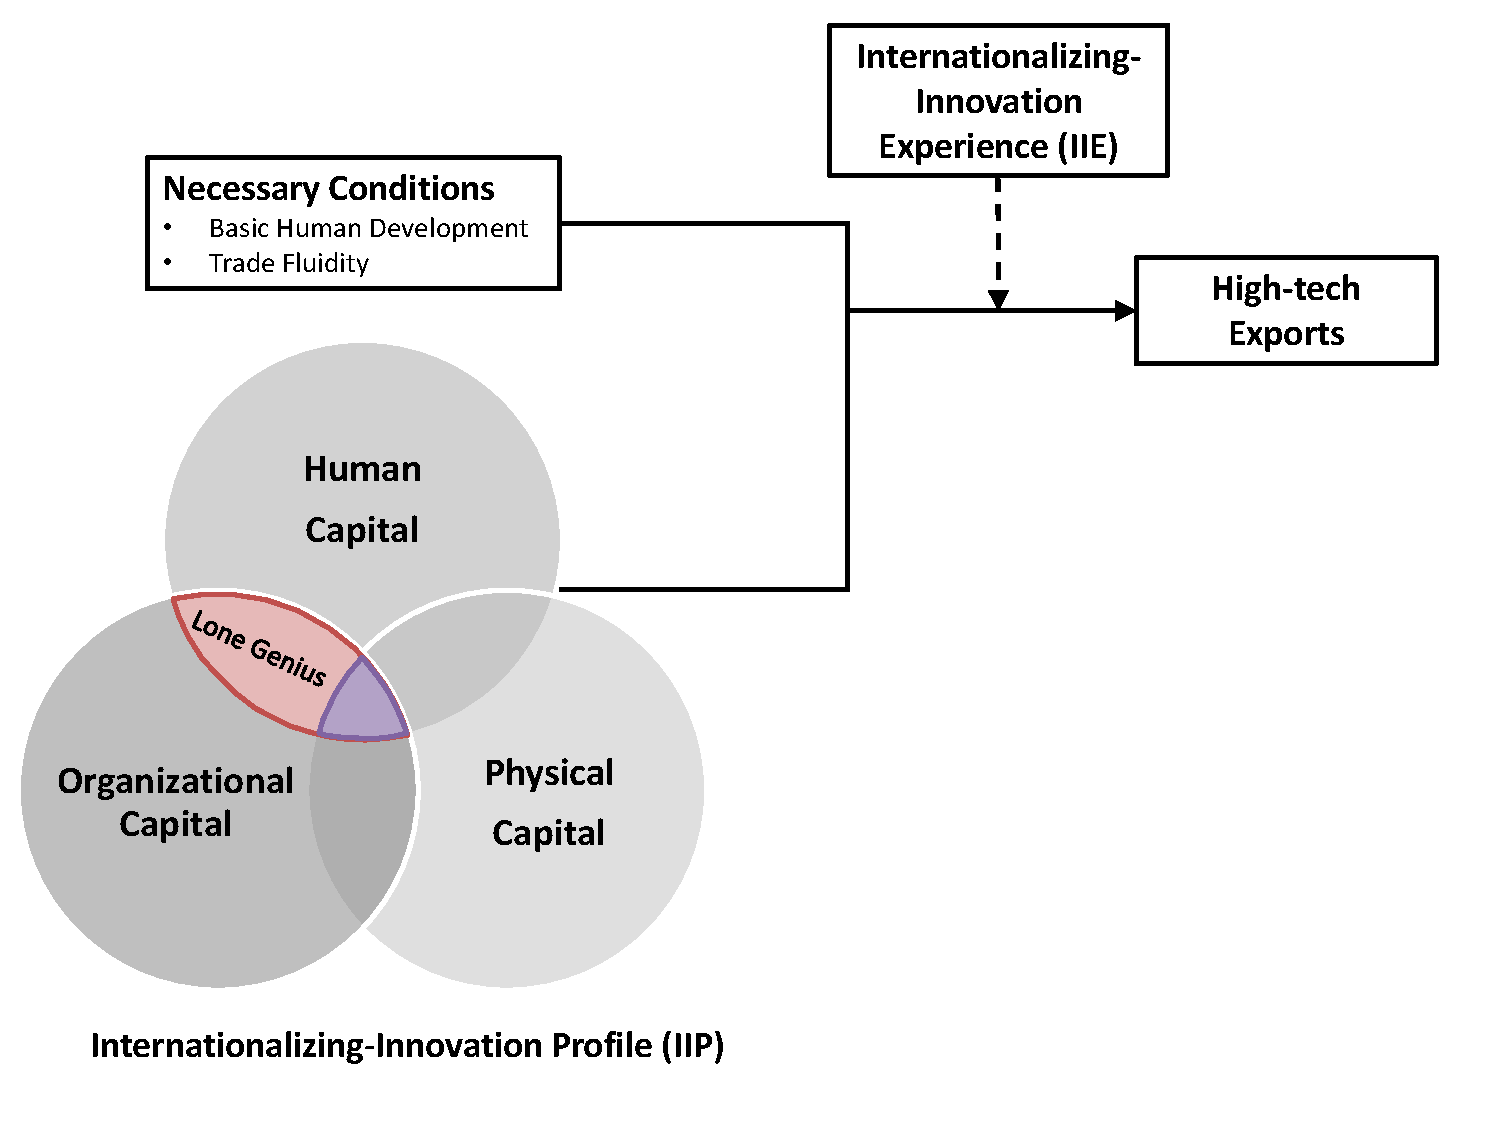
\includegraphics[trim = 0 0 0 0,clip,width=\textwidth]{figures/conceptual-model-v4.pdf} }
    \end{center}
    \label{fig:conceptual-model}
    \hrule
\end{figure}

See Figure \ref{fig:conceptual-model}.

\newpage

This is a
footnote\footnote{This is a footnote that can be really long.  \newline You can have multiple paragraphs in the footnote.  You can have \underline{underline} or \textbf{bold} or \emph{italics}.  You can even have a math equation inline. \newline In this section, we review the regression results to summarize our findings.  First, we examine each model for significance, and conclude the hypothesized models fit well with the data.  Second, we conclude that the fixed country effects represent consistent and unbiased parameter estimates.  Third, with the use of the \citet{Driscoll:1998} robust standard errors, we adjust any variance bias to ascertain the significance of these consistent estimates.  Therefore, we are able to make inferences about the hypotheses using our model estimates.  For ease of interpretation across these 12 models, we introduce $\betaSH{{ \ \ }M1}{Total}{1}$ as notation to refer to parameter estimate $\hat{\beta}_{1}$ (HDI) for the Total Sample and (M1) Model 1:  Main Effects.  We proceed by reporting findings for the total sample. \newline The footnotes are automatically converted to "endnotes" and will be included at the end of the document.  It will finish when you have that outer brace like this.}
that can be placed within a document.

\vspace{1.5in}

Refer to the Appendices in section\textasciitilde{}\ref{sec:appendix}
where I am going to cite John \citep[pp. 2-3]{Tukey:1962}.

Here is a quote by \citet[pp. 2-3]{Tukey:1962}:

\begin{quote}
For a long time I have thought I was a statistician, interested in inferences from the particular to the general.  But as I have watched mathematical statistics evolve, I have had to cause to wonder and to doubt. [...] All in all, I have come to feel that my central interest is in \emph{data analysis}, which I take to include among other things: procedures for analyzing data, techniques for interpreting the results of such procedures, ways of planning the gathering of data to make its analysis easier, more precise or more accurate, and all the machinery and results of (mathematical) statistics which apply to analyzing the data.

Large parts of data analysis are inferential in the sample-to-population sense, but these are only parts, not the whole.  Large parts of data analysis are incisive, laying bare indications which we could not perceive by simple and direct examination of the raw data, but these too are only parts, not the whole.  Some parts of data analysis, as the term is her stretch beyond its philology, are allocation, in the sense that they guide us in the distribution of effort and other valuable considerations in observation, experimentation, or analysis.  Data analysis is a larger and more varied field than inference, or incisive procedures, or allocation.

Statistics has contributed much to data analysis.  In the future it can, and in my view should, contribute more.  For such contributions to exist, and be valuable, it is not necessary that they be direct.  They need not provide new techniques, or better tables for old techniques, in order to influence the practice of data analysis.
\end{quote}

\newpage

\begin{sidewaystable}[!htbp]
\footnotesize
\centering
\caption{\textbf{Descriptive Statistics and Correlation Analysis}}
\label{table:correlation}
\begin{tabularx}{0.975\textwidth}{{r@{ \ \ } p{35mm} r@{}lp{.25mm} r@{}l p{.5mm} r@{}l p{.01mm} r@{}l p{.01mm} r@{}l p{.01mm} r@{}l p{.01mm} r@{}l p{.01mm} r@{}l p{.01mm} r@{}l p{.01mm} r@{}l p{.01mm} r@{}l p{.01mm} r@{}l p{.01mm} r@{}l p{.01mm}   r@{}l  }}
 & \\
\hline
 & \\
\multicolumn{2}{c}{\textbf{ }} & \multicolumn{2}{c}{\textbf{M}} & & \multicolumn{2}{c}{\textbf{SD}} &  & \multicolumn{2}{c}{\textbf{1}} &  & \multicolumn{2}{c}{\textbf{2}} &  & \multicolumn{2}{c}{\textbf{3}} &  & \multicolumn{2}{c}{\textbf{4}} &  & \multicolumn{2}{c}{\textbf{5}} &  & \multicolumn{2}{c}{\textbf{6}} &  & \multicolumn{2}{c}{\textbf{7}} &  & \multicolumn{2}{c}{\textbf{8}} &  & \multicolumn{2}{c}{\textbf{9}} &  & \multicolumn{2}{c}{\textbf{10}} &  & \multicolumn{2}{c}{\textbf{11}} &  & \\ 
 & \\
\hline
 & \\
\textbf{1} & \textbf{Height (cm)} &  167&.3 &  &  15&.24 &  &  \multicolumn{2}{c}{1}  &  &  \multicolumn{2}{c}{ \  \  \  \  \ }  &  &  \multicolumn{2}{c}{ \  \  \  \  \ }  &  &  \multicolumn{2}{c}{ \  \  \  \  \ }  &  &  \multicolumn{2}{c}{ \  \  \  \  \ }  &  &  \multicolumn{2}{c}{ \  \  \  \  \ }  &  &  \multicolumn{2}{c}{ \  \  \  \  \ }  &  &  \multicolumn{2}{c}{ \  \  \  \  \ }  &  &  \multicolumn{2}{c}{ \  \  \  \  \ }  &  &  \multicolumn{2}{c}{ \  \  \  \  \ }  &  &  \multicolumn{2}{c}{ \  \  \  \  \ }  &  & \\ 
 & \\
\textbf{2} & \textbf{Arm Span (cm)} &  167&.4 &  &  21&.54 &  &  &.72{$^{***}$}  &  &  \multicolumn{2}{c}{1}  &  &  \multicolumn{2}{c}{ \  \  \  \  \ }  &  &  \multicolumn{2}{c}{ \  \  \  \  \ }  &  &  \multicolumn{2}{c}{ \  \  \  \  \ }  &  &  \multicolumn{2}{c}{ \  \  \  \  \ }  &  &  \multicolumn{2}{c}{ \  \  \  \  \ }  &  &  \multicolumn{2}{c}{ \  \  \  \  \ }  &  &  \multicolumn{2}{c}{ \  \  \  \  \ }  &  &  \multicolumn{2}{c}{ \  \  \  \  \ }  &  &  \multicolumn{2}{c}{ \  \  \  \  \ }  &  & \\ 
 & \\
\textbf{3} & \textbf{Hand Length (cm)} &  19&.6 &  &  16&.82 &  &  &.15{$^{*}$}  &  &  &.11{$^{\dagger}$}  &  &  \multicolumn{2}{c}{1}  &  &  \multicolumn{2}{c}{ \  \  \  \  \ }  &  &  \multicolumn{2}{c}{ \  \  \  \  \ }  &  &  \multicolumn{2}{c}{ \  \  \  \  \ }  &  &  \multicolumn{2}{c}{ \  \  \  \  \ }  &  &  \multicolumn{2}{c}{ \  \  \  \  \ }  &  &  \multicolumn{2}{c}{ \  \  \  \  \ }  &  &  \multicolumn{2}{c}{ \  \  \  \  \ }  &  &  \multicolumn{2}{c}{ \  \  \  \  \ }  &  & \\ 
 & \\
\textbf{4} & \textbf{Hand to Elbow (cm)} &  42&.5 &  &  4&.60 &  &  &.70{$^{***}$}  &  &  &.60{$^{***}$}  &  &  &.10 &  &  \multicolumn{2}{c}{1}  &  &  \multicolumn{2}{c}{ \  \  \  \  \ }  &  &  \multicolumn{2}{c}{ \  \  \  \  \ }  &  &  \multicolumn{2}{c}{ \  \  \  \  \ }  &  &  \multicolumn{2}{c}{ \  \  \  \  \ }  &  &  \multicolumn{2}{c}{ \  \  \  \  \ }  &  &  \multicolumn{2}{c}{ \  \  \  \  \ }  &  &  \multicolumn{2}{c}{ \  \  \  \  \ }  &  & \\ 
 & \\
\textbf{5} & \textbf{Elbow to Armpit (cm)} &  26&.7 &  &  6&.47 &  &  &.39{$^{***}$}  &  &  &.27{$^{***}$}  &  &  &.05 &  &  &.42{$^{***}$}  &  &  \multicolumn{2}{c}{1}  &  &  \multicolumn{2}{c}{ \  \  \  \  \ }  &  &  \multicolumn{2}{c}{ \  \  \  \  \ }  &  &  \multicolumn{2}{c}{ \  \  \  \  \ }  &  &  \multicolumn{2}{c}{ \  \  \  \  \ }  &  &  \multicolumn{2}{c}{ \  \  \  \  \ }  &  &  \multicolumn{2}{c}{ \  \  \  \  \ }  &  & \\ 
 & \\
\textbf{6} & \textbf{Floor to Kneepit (cm)} &  191&.6 &  &  49&.68 &  &  &.28{$^{***}$}  &  &  &.27{$^{***}$}  &  &  &.08 &  &  &.09 &  &  -&.03 &  &  \multicolumn{2}{c}{1}  &  &  \multicolumn{2}{c}{ \  \  \  \  \ }  &  &  \multicolumn{2}{c}{ \  \  \  \  \ }  &  &  \multicolumn{2}{c}{ \  \  \  \  \ }  &  &  \multicolumn{2}{c}{ \  \  \  \  \ }  &  &  \multicolumn{2}{c}{ \  \  \  \  \ }  &  & \\ 
 & \\
\textbf{7} & \textbf{Floor to Hip (cm)} &  24&.8 &  &  2&.69 &  &  &.71{$^{***}$}  &  &  &.60{$^{***}$}  &  &  &.08 &  &  &.58{$^{***}$}  &  &  &.29{$^{***}$}  &  &  &.30{$^{***}$}  &  &  \multicolumn{2}{c}{1}  &  &  \multicolumn{2}{c}{ \  \  \  \  \ }  &  &  \multicolumn{2}{c}{ \  \  \  \  \ }  &  &  \multicolumn{2}{c}{ \  \  \  \  \ }  &  &  \multicolumn{2}{c}{ \  \  \  \  \ }  &  & \\ 
 & \\
\textbf{8} & \textbf{Floor to Armpit (cm)} &  45&.2 &  &  5&.24 &  &  &.70{$^{***}$}  &  &  &.43{$^{***}$}  &  &  &.10 &  &  &.53{$^{***}$}  &  &  &.32{$^{***}$}  &  &  &.17{$^{*}$}  &  &  &.52{$^{***}$}  &  &  \multicolumn{2}{c}{1}  &  &  \multicolumn{2}{c}{ \  \  \  \  \ }  &  &  \multicolumn{2}{c}{ \  \  \  \  \ }  &  &  \multicolumn{2}{c}{ \  \  \  \  \ }  &  & \\ 
 & \\
\textbf{9} & \textbf{NA} &  95&.3 &  &  9&.51 &  &  &.71{$^{***}$}  &  &  &.50{$^{***}$}  &  &  &.10 &  &  &.53{$^{***}$}  &  &  &.27{$^{***}$}  &  &  &.26{$^{***}$}  &  &  &.56{$^{***}$}  &  &  &.54{$^{***}$}  &  &  \multicolumn{2}{c}{1}  &  &  \multicolumn{2}{c}{ \  \  \  \  \ }  &  &  \multicolumn{2}{c}{ \  \  \  \  \ }  &  & \\ 
 & \\
\textbf{10} & \textbf{NA} &  131&.3 &  &  11&.90 &  &  &.88{$^{***}$}  &  &  &.57{$^{***}$}  &  &  &.14{$^{*}$}  &  &  &.68{$^{***}$}  &  &  &.37{$^{***}$}  &  &  &.31{$^{***}$}  &  &  &.66{$^{***}$}  &  &  &.63{$^{***}$}  &  &  &.77{$^{***}$}  &  &  \multicolumn{2}{c}{1}  &  &  \multicolumn{2}{c}{ \  \  \  \  \ }  &  & \\ 
 & \\
\textbf{11} & \textbf{NA} &  7&.6 &  &  &.87 &  &  &.43{$^{***}$}  &  &  &.40{$^{***}$}  &  &  &.13{$^{*}$}  &  &  &.29{$^{***}$}  &  &  &.22{$^{***}$}  &  &  &.12{$^{\dagger}$}  &  &  &.22{$^{***}$}  &  &  &.21{$^{**}$}  &  &  &.28{$^{***}$}  &  &  &.34{$^{***}$}  &  &  \multicolumn{2}{c}{1}  &  & \\ 
 & \\
\textbf{12} & \textbf{NA} &  50&.5 &  &  9&.61 &  &  &.65{$^{***}$}  &  &  &.45{$^{***}$}  &  &  &.11 &  &  &.41{$^{***}$}  &  &  &.26{$^{***}$}  &  &  &.21{$^{**}$}  &  &  &.38{$^{***}$}  &  &  &.38{$^{***}$}  &  &  -&.04 &  &  &.43{$^{***}$}  &  &  &.56{$^{***}$}  &  & \\ 
 & \\
\hline
 & \\
\multicolumn{40}{p{0.88\textwidth}}{  \footnotesize { \begin{hangparas}{0.75in}{1} \textbf{\underline{Notes}:} \ \ Pearson pairwise correlations are reported; \newline a two-side test was 
  performed to report correlation significance.  \end{hangparas} } }  & \\  
\multicolumn{40}{p{0.88\textwidth}}{  {\tiny {$^{\dagger} p < .10$} }  {     } {\tiny        {$^{*} p < .05$} }  {     } {\tiny       {$^{**} p < .01$} }  {     } {\tiny      {$^{***} p < .001$} } {     }     } & \\ 
 & \\
\hline
\end{tabularx}
\end{sidewaystable}


\newpage

\newpage
\section{APPENDICES}
\label{sec:appendix}

\subsection{Data Provenance}
\label{sec:appendix-data-provenance}

\newpage
\subsubsection{Data Collection Handout}
\label{sec:appendix-data-handout}

\begin{figure}[!ht]
    \hrule
    \caption{ \textbf{Handout Page 1} }
    \begin{center}
        \scalebox{1.00}{    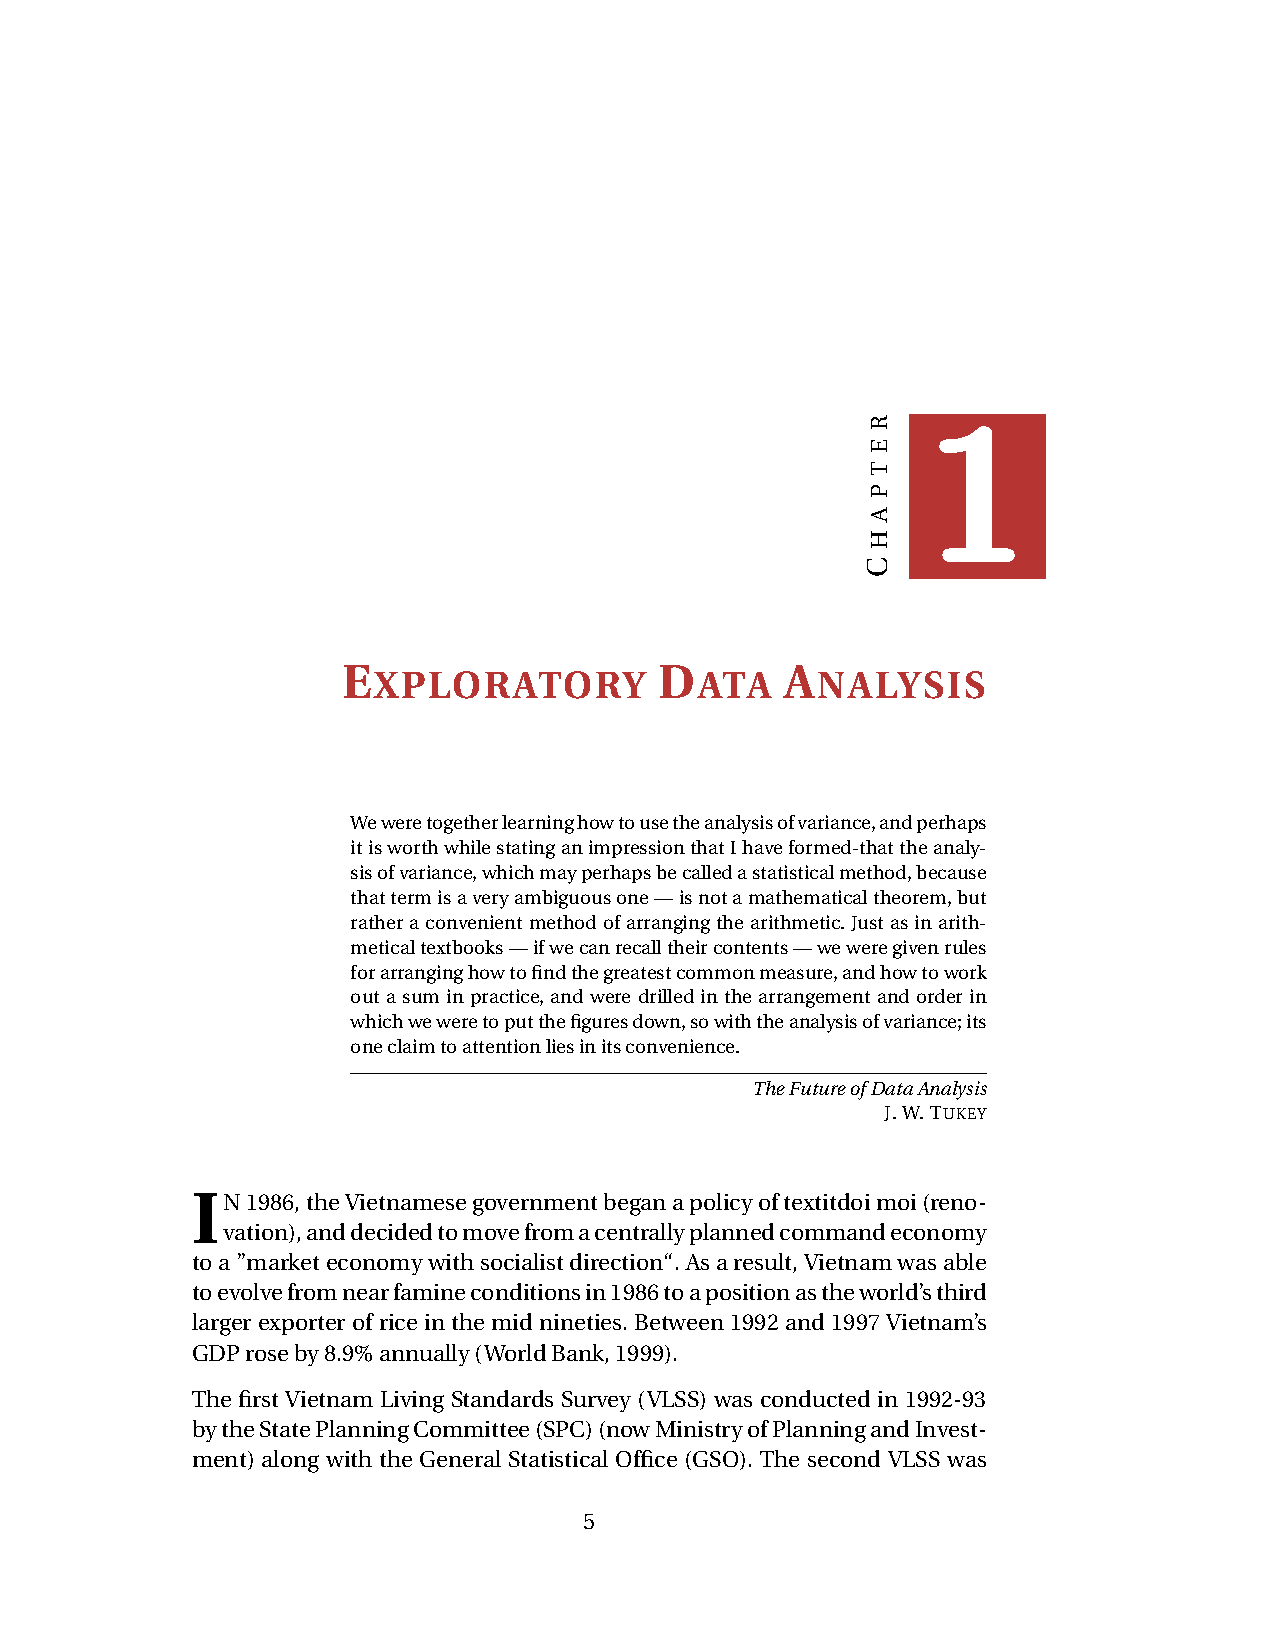
\includegraphics[trim = 0 0 0 0,clip,width=0.85\textwidth]{pdfs/handout1.pdf} }
    \end{center}
    \label{fig:handout-1}
    \hrule
\end{figure}

\newpage

\begin{figure}[!ht]
    \hrule
    \caption{ \textbf{Handout Page 2} }
    \begin{center}
        \scalebox{1.00}{    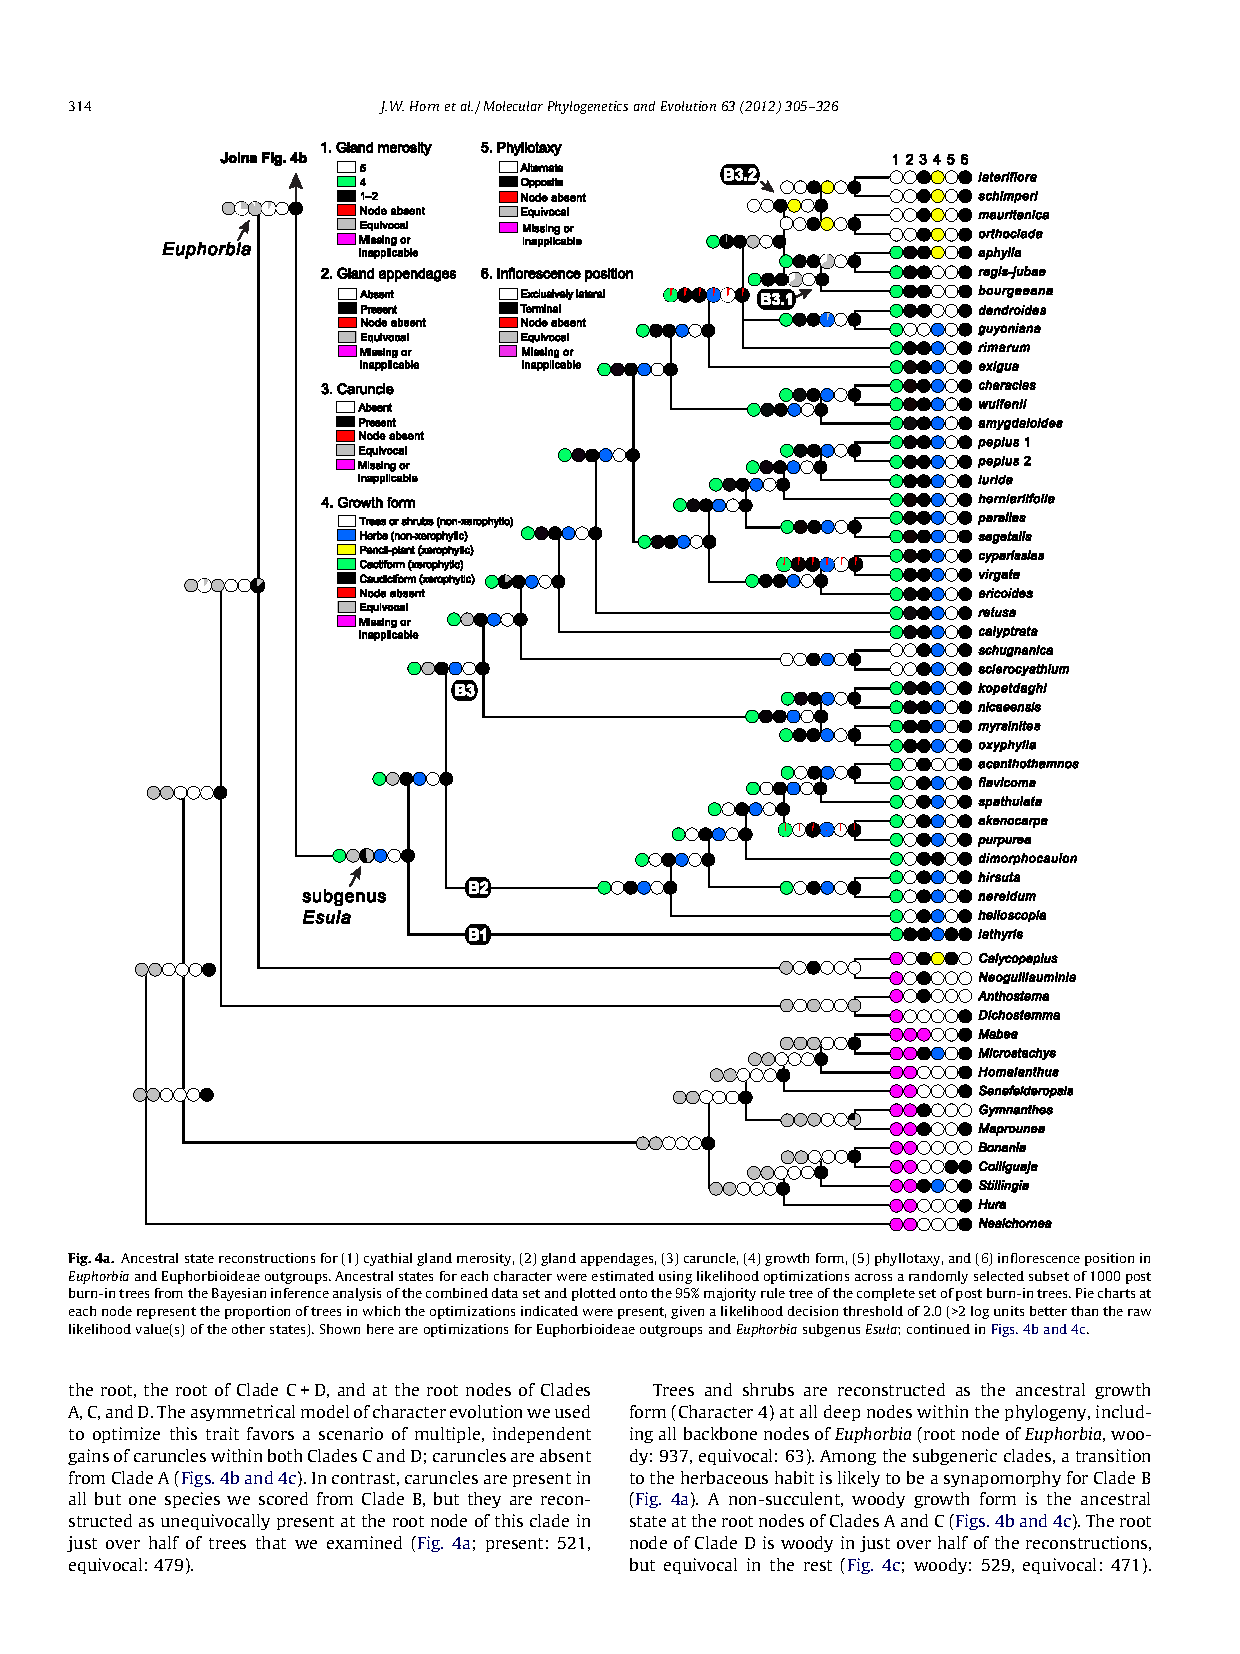
\includegraphics[trim = 0 0 0 0,clip,width=0.85\textwidth]{pdfs/handout2.pdf} }
    \end{center}
    \label{fig:handout-2}
    \hrule
\end{figure}

\newpage

\begin{figure}[!ht]
    \begin{subfigure}[h]{0.5\textwidth}
    \centering
    % trim={<left> <lower> <right> <upper>}
    % https://shantoroy.com/latex/add-subfig-in-latex/
    % male figure
            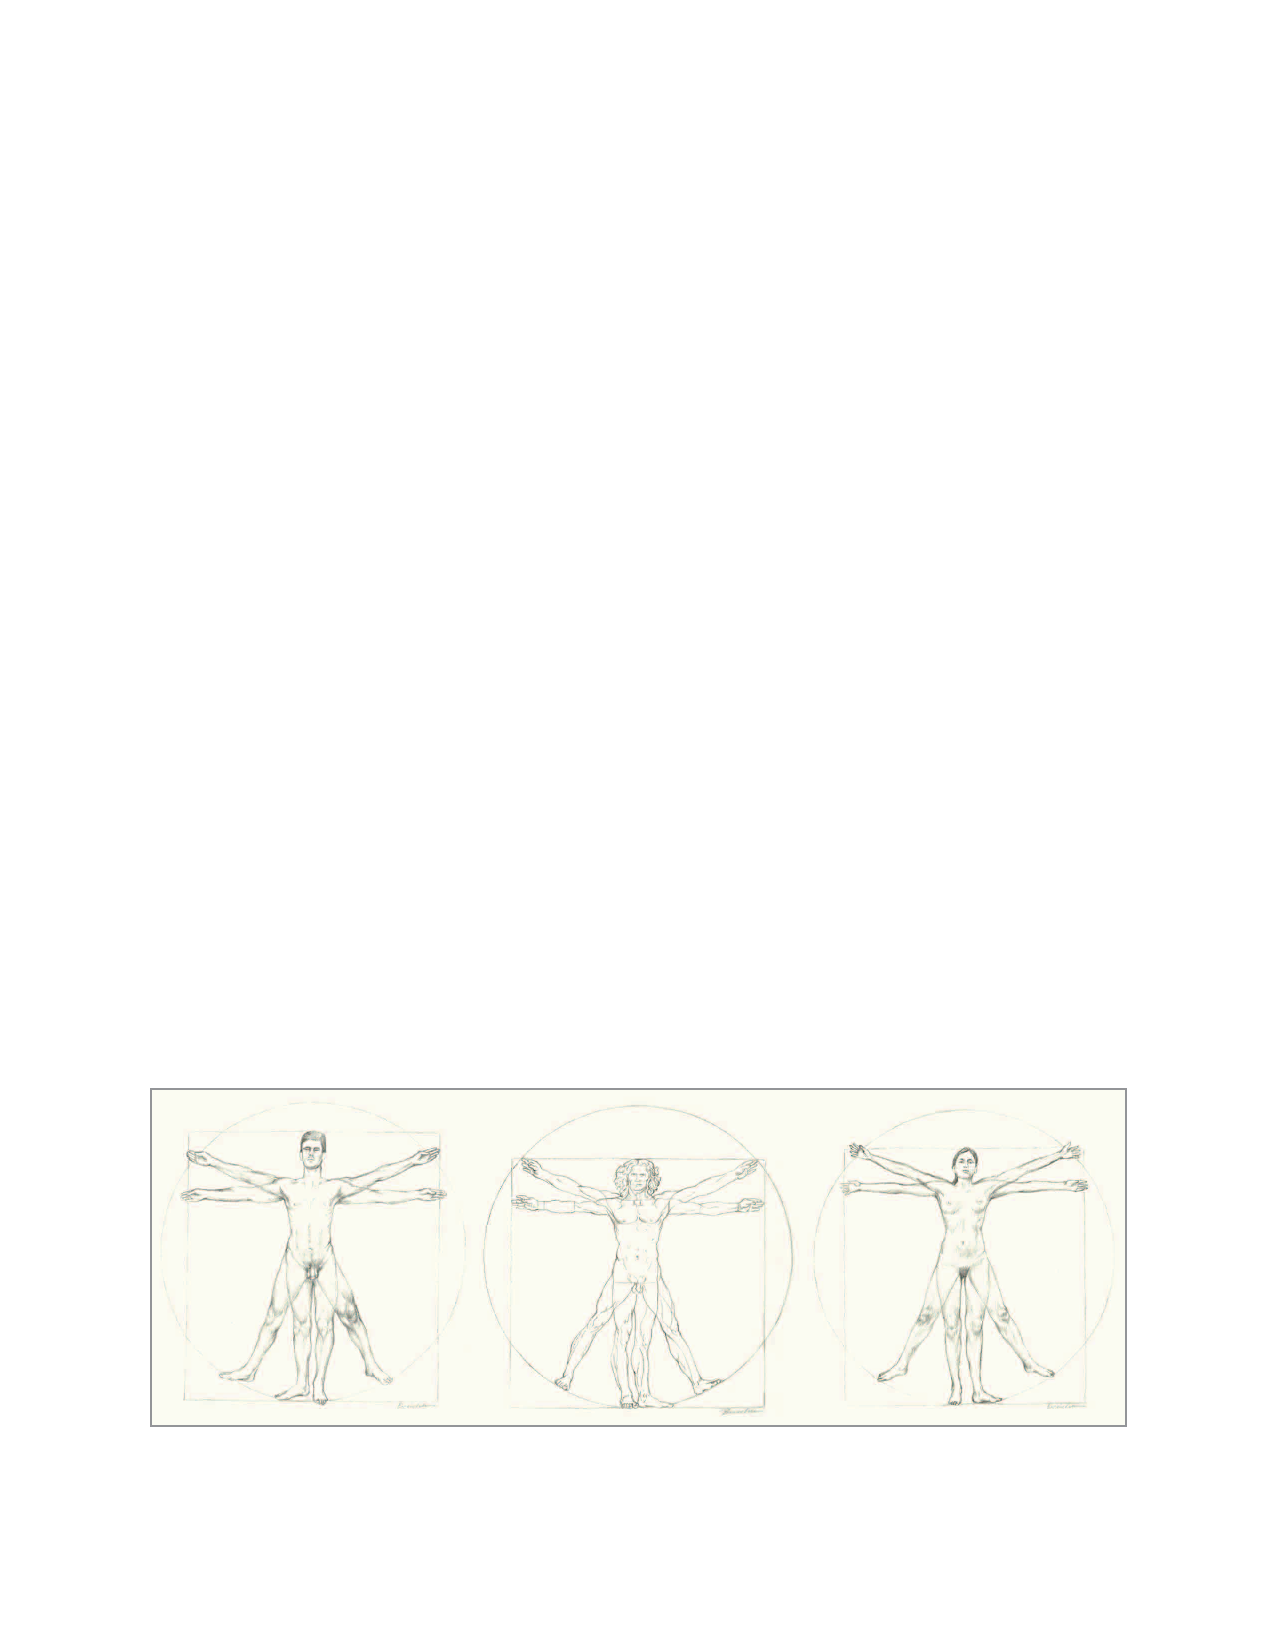
\includegraphics[trim = 0 0 11.25cm 0,clip,scale=1]{figures/Vitruvian.pdf}
        \caption{ \citet{Thomas:2020} discuss this. }
        \label{fig:sub-first}
    \end{subfigure}
    \begin{subfigure}[h]{0.5\textwidth}
    \centering
    % female figure
        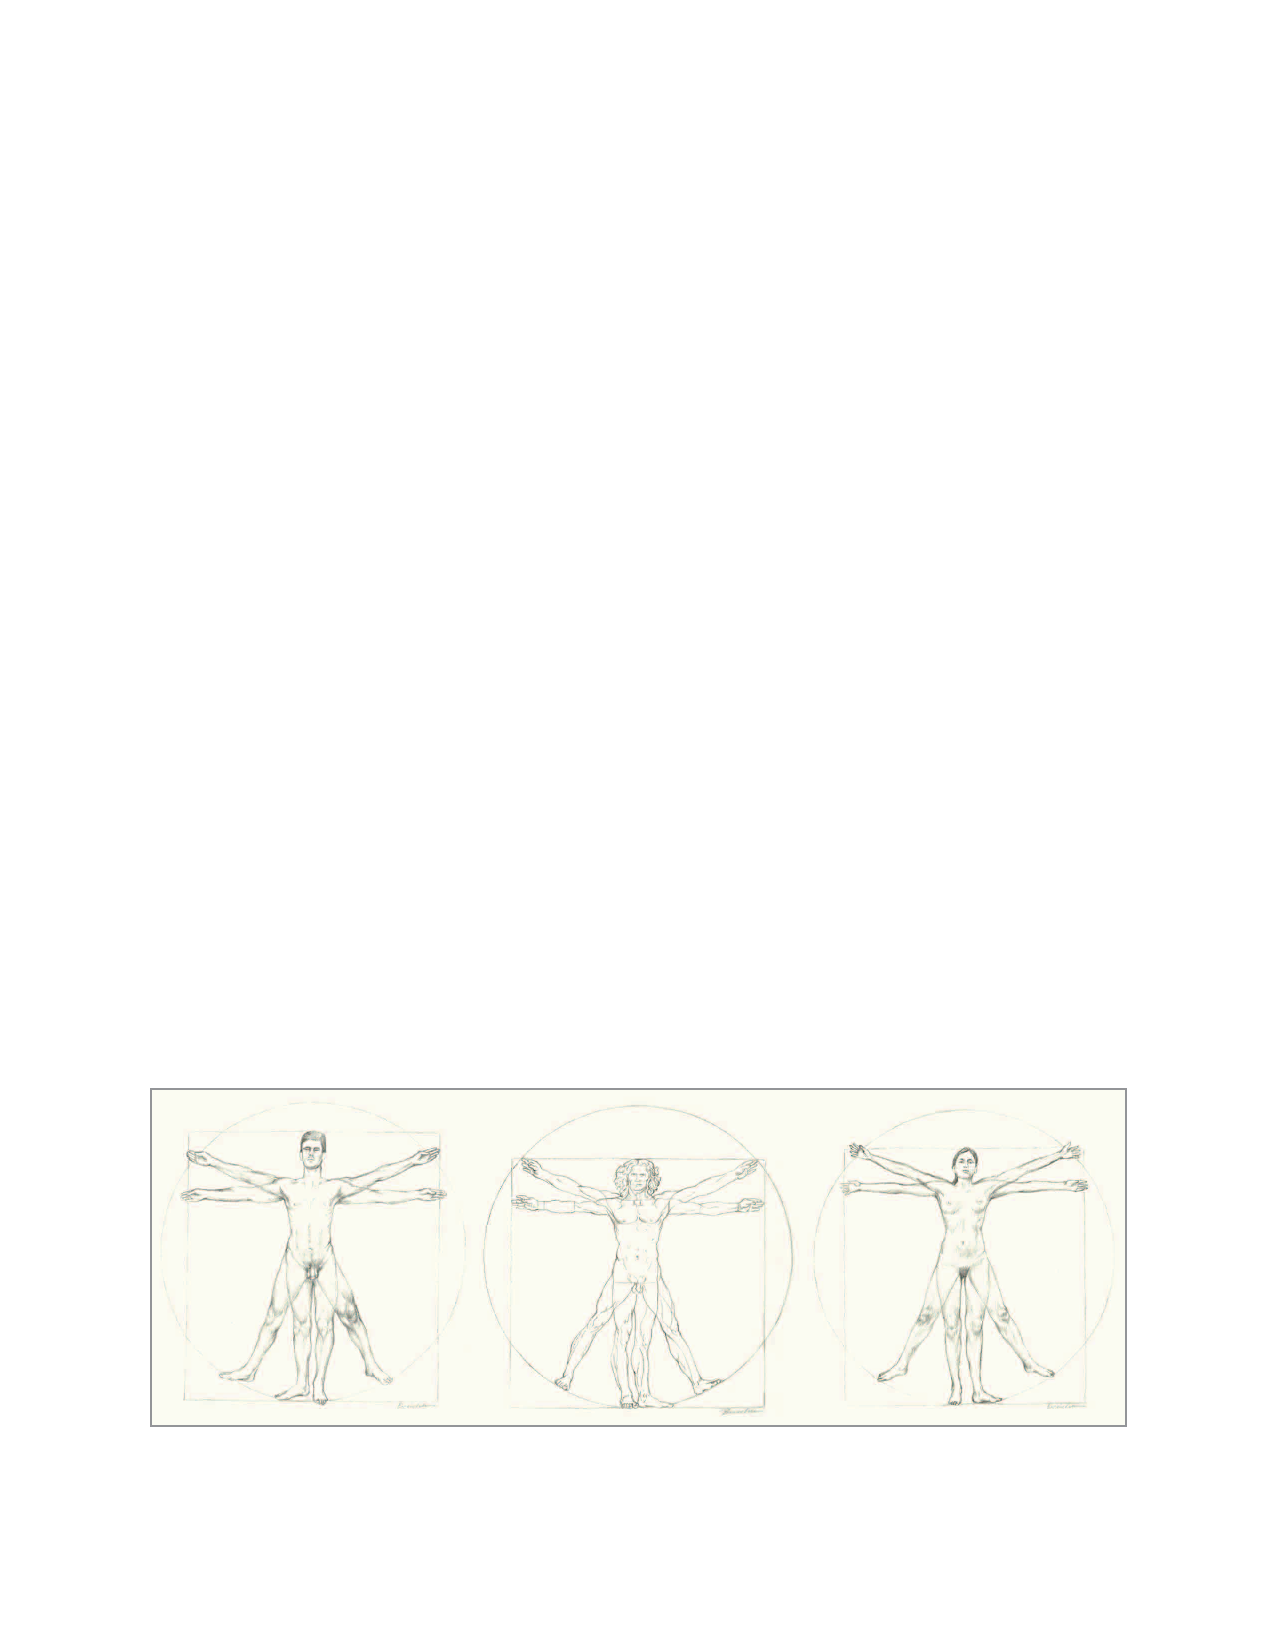
\includegraphics[trim = 11.25cm 0 0 0,clip,scale=1]{figures/Vitruvian.pdf}
            \caption{Schnitt realer Sensor \citep{Thomas:2020}}
        \label{fig:sub-second}
    \end{subfigure}
    \vspace{2.5mm}
    \hrule
    \vspace{2.5mm}
        \caption{\textbf{ Der Sensor in Theorie und Verwirklichung... caption at bottom instead? }  I can write a really long caption if I want. \newline This is using "crop" to include one image and trim it to appear as two.  Likely you will have two separate images if you use this option, so you would set the trim parameters all equal to 0.  \newline   This figure has subfigures which each also have a possible caption.   }
        \label{fig:combined}
    \vspace{-2.5mm}
    \hrule
\end{figure}

\newpage

\subsection{Preparing the Report Workspace as a subsection}
\label{sec:appendix-setup}

\subsubsection{Preparing the Report Workspace as a subsubsection}
\label{sec:appendix-setup2}

\paragraph{Preparing the Report Workspace as a paragraph}
\label{sec:appendix-setup3}

\subparagraph{Preparing the Report Workspace as a subparagrah}
\label{sec:appendix-setup4}

Below is the necessary functions and libraries required to run the code
referenced in this document.

\begin{Shaded}
\begin{Highlighting}[]
\KeywordTok{library}\NormalTok{(devtools); }\CommentTok{# required for source_url}

\NormalTok{path.humanVerseWSU =}\StringTok{ "https://raw.githubusercontent.com/MonteShaffer/humanVerseWSU/"}
\KeywordTok{source_url}\NormalTok{( }\KeywordTok{paste0}\NormalTok{(path.humanVerseWSU,}\StringTok{"master/misc/functions-project-measure.R"}\NormalTok{) );}
\end{Highlighting}
\end{Shaded}

Below is the code to load the data and prepare it for analysis.

\begin{Shaded}
\begin{Highlighting}[]
\NormalTok{path.to.project =}\StringTok{ "C:/Users/Connor/.ssh/stats419/project-measure/"}\NormalTok{;}
\NormalTok{path.to.secret =}\StringTok{ }
\StringTok{  "C:/Users/Connor/Documents/1) WSU 2018-/Fall 2020/Stat 419/Project 1 Measure/"}\NormalTok{;}
\NormalTok{path.to.tables =}\StringTok{ }\KeywordTok{paste0}\NormalTok{(path.to.project,}\StringTok{"tables/"}\NormalTok{);}
  \KeywordTok{createDirRecursive}\NormalTok{(path.to.tables);}

\NormalTok{measure =}\StringTok{ }\NormalTok{utils}\OperatorTok{::}\KeywordTok{read.csv}\NormalTok{( }\KeywordTok{paste0}\NormalTok{(path.to.secret, }\StringTok{"cm.final.measure.txt"}\NormalTok{), }\DataTypeTok{header=}\OtherTok{TRUE}\NormalTok{, }
                          \DataTypeTok{quote=}\StringTok{""}\NormalTok{, }\DataTypeTok{sep=}\StringTok{"|"}\NormalTok{);}

\NormalTok{path.github =}\StringTok{ "https://raw.githubusercontent.com/youknowwwho/stats419/"}\NormalTok{;}
\KeywordTok{source_url}\NormalTok{( }\KeywordTok{paste0}\NormalTok{(path.github,}\StringTok{"master/Functions/functions-project-measure.R"}\NormalTok{) );}

\NormalTok{prepareMeasureData2 =}\StringTok{ }\ControlFlowTok{function}\NormalTok{(myData)\{}
  
\NormalTok{  newData =}\StringTok{ }\NormalTok{myData;}
  
\NormalTok{  newData}\OperatorTok{$}\NormalTok{my.eye[newData}\OperatorTok{$}\NormalTok{eye }\OperatorTok{==}\StringTok{ "}\CharTok{\textbackslash{}"}\StringTok{left}\CharTok{\textbackslash{}"}\StringTok{"} \OperatorTok{&}\StringTok{ }\NormalTok{newData}\OperatorTok{$}\NormalTok{my.eye }\OperatorTok{==}\StringTok{ "r"}\NormalTok{] =}\StringTok{ "l"}\NormalTok{; }
\NormalTok{  newData}\OperatorTok{$}\NormalTok{minutes[newData}\OperatorTok{$}\NormalTok{minutes }\OperatorTok{<=}\StringTok{ }\DecValTok{0}\NormalTok{] =}\StringTok{ }\OtherTok{NA}\NormalTok{;}
  
  \KeywordTok{return}\NormalTok{(newData);}
\NormalTok{\}}

\KeywordTok{set.seed}\NormalTok{(}\DecValTok{11906189}\NormalTok{);}

\NormalTok{measure.df =}\StringTok{ }\KeywordTok{prepareMeasureData2}\NormalTok{(measure);}

\KeywordTok{summary}\NormalTok{(measure.df);}
\end{Highlighting}
\end{Shaded}

\begin{verbatim}
##  data_collector      person_id             height        head.height   
##  Length:251         Length:251         Min.   : 85.09   Min.   :15.24  
##  Class :character   Class :character   1st Qu.:160.00   1st Qu.:20.50  
##  Mode  :character   Mode  :character   Median :168.40   Median :22.00  
##                                        Mean   :167.25   Mean   :22.24  
##                                        3rd Qu.:177.80   3rd Qu.:23.50  
##                                        Max.   :191.10   Max.   :38.10  
##                                        NA's   :9        NA's   :9      
##  head.circumference    arm.span      floor.navel       units          
##  Min.   :21.50      Min.   : 61.5   Min.   : 49.0   Length:251        
##  1st Qu.:55.00      1st Qu.:158.9   1st Qu.: 95.0   Class :character  
##  Median :56.58      Median :168.9   Median :101.0   Mode  :character  
##  Mean   :56.08      Mean   :167.4   Mean   :101.6                     
##  3rd Qu.:58.42      3rd Qu.:179.0   3rd Qu.:107.0                     
##  Max.   :64.10      Max.   :224.0   Max.   :151.1                     
##  NA's   :19         NA's   :8       NA's   :50                        
##    writing              eye             eye.color           swinging        
##  Length:251         Length:251         Length:251         Length:251        
##  Class :character   Class :character   Class :character   Class :character  
##  Mode  :character   Mode  :character   Mode  :character   Mode  :character  
##                                                                             
##                                                                             
##                                                                             
##                                                                             
##       age           gender             quality          minutes     
##  Min.   : 1.00   Length:251         Min.   : 5.000   Min.   : 2.00  
##  1st Qu.:22.00   Class :character   1st Qu.: 8.000   1st Qu.:10.00  
##  Median :27.00   Mode  :character   Median : 9.000   Median :15.00  
##  Mean   :34.69                      Mean   : 8.616   Mean   :15.96  
##  3rd Qu.:50.00                      3rd Qu.:10.000   3rd Qu.:20.00  
##  Max.   :94.00                      Max.   :10.000   Max.   :45.00  
##                                                      NA's   :21     
##   ethnicity            notes            hand.length       hand.width   
##  Length:251         Length:251         Min.   :  9.00   Min.   : 7.00  
##  Class :character   Class :character   1st Qu.: 17.00   1st Qu.:18.48  
##  Mode  :character   Mode  :character   Median : 18.00   Median :20.00  
##                                        Mean   : 19.64   Mean   :19.69  
##                                        3rd Qu.: 19.50   3rd Qu.:21.59  
##                                        Max.   :223.20   Max.   :26.50  
##                                        NA's   :13       NA's   :23     
##    hand.elbow    elbow.armpit     arm.reach      foot.length    floor.kneepit  
##  Min.   :23.0   Min.   :10.00   Min.   : 38.0   Min.   :13.50   Min.   :23.00  
##  1st Qu.:40.0   1st Qu.:23.00   1st Qu.:193.0   1st Qu.:23.00   1st Qu.:42.00  
##  Median :43.0   Median :26.00   Median :207.0   Median :24.77   Median :45.09  
##  Mean   :42.5   Mean   :26.72   Mean   :191.6   Mean   :24.77   Mean   :45.20  
##  3rd Qu.:45.5   3rd Qu.:29.21   3rd Qu.:221.6   3rd Qu.:26.40   3rd Qu.:48.26  
##  Max.   :52.0   Max.   :71.00   Max.   :245.0   Max.   :38.10   Max.   :72.20  
##  NA's   :23     NA's   :24      NA's   :24      NA's   :22      NA's   :22     
##    floor.hip       floor.armpit     my.units         my.ethnicity      
##  Min.   : 35.00   Min.   : 70.0   Length:251         Length:251        
##  1st Qu.: 91.40   1st Qu.:124.5   Class :character   Class :character  
##  Median : 96.00   Median :131.5   Mode  :character   Mode  :character  
##  Mean   : 95.29   Mean   :131.3                                        
##  3rd Qu.:101.00   3rd Qu.:139.7                                        
##  Max.   :113.00   Max.   :156.8                                        
##  NA's   :34       NA's   :22                                           
##   my.gender          new.units            my.eye           my.writing       
##  Length:251         Length:251         Length:251         Length:251        
##  Class :character   Class :character   Class :character   Class :character  
##  Mode  :character   Mode  :character   Mode  :character   Mode  :character  
##                                                                             
##                                                                             
##                                                                             
##                                                                             
##  my.swinging        my.eye.color      
##  Length:251         Length:251        
##  Class :character   Class :character  
##  Mode  :character   Mode  :character  
##                                       
##                                       
##                                       
## 
\end{verbatim}

Below is the code to generate the summary statistics and save them as a
table that you see in Section \ref{}.

\begin{Shaded}
\begin{Highlighting}[]
\KeywordTok{set.seed}\NormalTok{(}\DecValTok{11906189}\NormalTok{);}

\NormalTok{measure.df.numeric =}\StringTok{ }\NormalTok{measure.df[}\KeywordTok{sapply}\NormalTok{(measure.df, is.numeric)]; }\CommentTok{#Help From:}
\CommentTok{#https://www.statology.org/calculate-mean-multiple-columns-in-r/#:~:text=Often%20you%20}
\CommentTok{#may%20want%20to,using%20the%20colMeans()%20function.}

\NormalTok{my.Means =}\StringTok{ }\KeywordTok{colMeans}\NormalTok{(measure.df.numeric, }\DataTypeTok{na.rm =} \OtherTok{TRUE}\NormalTok{); }\CommentTok{#get mean of each column}
\NormalTok{my.StanDevs =}\StringTok{ }\KeywordTok{sapply}\NormalTok{(measure.df.numeric, sd, }\DataTypeTok{na.rm =} \OtherTok{TRUE}\NormalTok{); }\CommentTok{#get stan dev of each column}

\NormalTok{file.correlation =}\StringTok{ }\KeywordTok{paste0}\NormalTok{(path.to.tables,}\StringTok{"correlation-table1.tex"}\NormalTok{); }\CommentTok{#save table name as}

\NormalTok{myData =}\StringTok{ }\KeywordTok{as.matrix}\NormalTok{(measure.df.numeric[}\OperatorTok{-}\KeywordTok{c}\NormalTok{(}\DecValTok{2}\OperatorTok{:}\DecValTok{3}\NormalTok{,}\DecValTok{5}\OperatorTok{:}\DecValTok{8}\NormalTok{,}\DecValTok{10}\NormalTok{)]);  }\CommentTok{#numeric values minus }
\CommentTok{#head.height (2), head.circumference (3), navel.floor (5), age (6) quality (7), }
\CommentTok{#minutes (8), and hand.width (10)}

\CommentTok{# https://www.overleaf.com/read/srzhrcryjpwn}
\CommentTok{# keepaspectratio of include graphics }
\CommentTok{# could scale \textbackslash{}input if still too big ...}
\CommentTok{# https://tex.stackexchange.com/questions/13460/scalebox-knowing-how-much-it-scales#13487}

\KeywordTok{buildLatexCorrelationTable}\NormalTok{(myData, }
  \DataTypeTok{rotateTable =} \OtherTok{TRUE}\NormalTok{,}
  \DataTypeTok{width.table =} \FloatTok{.975}\NormalTok{,}
  \DataTypeTok{width.names =} \StringTok{"35mm"}\NormalTok{,}
  \DataTypeTok{space.M.SD =} \StringTok{".25mm"}\NormalTok{,}
  \DataTypeTok{space.SD.corr =} \StringTok{".5mm"}\NormalTok{,}
  \DataTypeTok{space.between =} \StringTok{".01mm"}\NormalTok{,}
  \DataTypeTok{myFile =}\NormalTok{ file.correlation,}
  \DataTypeTok{myNames =} \KeywordTok{c}\NormalTok{(}\StringTok{"Height (cm)"}\NormalTok{, }\StringTok{"Arm Span (cm)"}\NormalTok{, }\StringTok{"Hand Length (cm)"}\NormalTok{, }\StringTok{"Hand to Elbow (cm)"}\NormalTok{, }
              \StringTok{"Elbow to Armpit (cm)"}\NormalTok{, }\StringTok{"Arm Reach (cm)"}\NormalTok{, }\StringTok{"Foot Length (cm)"}\NormalTok{, }
              \StringTok{"Floor to Kneepit (cm)"}\NormalTok{, }\StringTok{"Floor to Hip (cm)"}\NormalTok{, }\StringTok{"Floor to Armpit (cm)"}\NormalTok{),}
  \DataTypeTok{myNote =} \StringTok{"Pearson pairwise correlations are reported; }\CharTok{\textbackslash{}\textbackslash{}}\StringTok{newline a two-side test was }
\StringTok{  performed to report correlation significance."}\NormalTok{,}
  \DataTypeTok{showOnes =} \StringTok{"center"}\NormalTok{);}

\KeywordTok{Sys.sleep}\NormalTok{(}\DecValTok{2}\NormalTok{); }\CommentTok{# in case Knit-PDF doesn't like that I just created the file...}
\end{Highlighting}
\end{Shaded}




%% appendices go here!


\newpage
\theendnotes

%%%%%%%%%%%%%%%%%%%%%%%%%%%%%%%%%%%  biblio %%%%%%%%
\newpage
\begin{auxmulticols}{2}
\singlespacing 
\bibliography{./../biblio/master.bib}

%%%%%%%%%%%%%%%%%%%%%%%%%%%%%%%%%%%  biblio %%%%%%%%
\end{auxmulticols}

\newpage
{
\hypersetup{linkcolor=black}
\setcounter{tocdepth}{3}
\tableofcontents
}



\end{document}